\documentclass{beamer}
% \usepackage{animate}
\usepackage{multimedia}

\usepackage{pgfpages}
\setbeameroption{show notes on second screen}
%https://tug.ctan.org/macros/latex/contrib/beamer/doc/beameruserguide.pdf

\usepackage[T2A]{fontenc}
\usepackage[utf8]{inputenc}
\usepackage[english,russian]{babel}
\usepackage{amsmath}
\usepackage{textcomp}
% \usepackage{hyperref}
% \usepackage{bookmark}
\hypersetup{unicode=true}

\setbeamertemplate{caption}[numbered]

\usetheme{CambridgeUS}
\usecolortheme{dolphin}


\title[Наблюдение и проецирование]{Преобразования наблюдения и проецирования}
\author[Быковских Д.А.]{Быковских Дмитрий Александрович}
\date{12.10.2024}

\begin{document}
	\begin{frame}
		\titlepage
	\end{frame}

	\section{Введение}

	\begin{frame}{Преобразования наблюдения и проецирования}
		Функции из библиотеки glm
		\begin{itemize}
			\item glm::lookAt(glm::vec3 position, glm::vec3 target, glm::vec3 up);
			\item glm::ortho(float left, float right, float bottom, float top, float near, float far);
			\item glm::perspective(float fovy, float aspect, float near, float far);
			\item glm::frustum(float left, float right, float bottom, float top, float near, float far);
		\end{itemize}
	\end{frame}

	\section{Преобразование наблюдения}
	\begin{frame}{Преобразование наблюдения}
		
		glm::lookAt(glm::vec3 position, glm::vec3 target, glm::vec3 up);

		Аргументы функции
		\begin{enumerate}
			\item position --- точка наблюдения;
			\item target --- базовая точка нашей сцены;
			% \item Выбирается направление наблюдения  (вектор нормали к плоскости наблюдения $target$).
			\item up --- вектор верха.
		\end{enumerate}
		
		\note{
			\begin{figure} 
				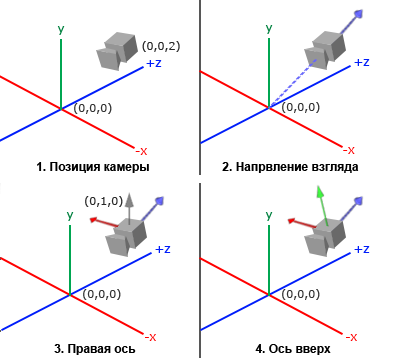
\includegraphics[width=0.55\textwidth]{images/camera_steps.png}
				\caption{Этапы преобразования наблюдения}
			\end{figure}
		}
	\end{frame}

	% https://www.khronos.org/opengl/wiki/GluLookAt_code
	
	\begin{frame}{Преобразования наблюдения}

		\begin{columns}
			\begin{column}{0.4\textwidth}
				\[
					n = \frac{N}{|N|}	= (n_x, n_y, n_z)
				\]
				\[
					u = \frac{V \times n }{|V|} = (v_x,v_y,v_z)	
				\]
		
				\[
					v = n \times u = (v_x, v_y, v_z)	
				\]
		
			\end{column}
			\begin{column}{0.6\textwidth}
				// 1. Вычисление направление наблюдения;

				glm::vec3 zaxis = glm::normalize(position - target);
				
				// 2. Вычисления направления вправо;
				
				glm::vec3 xaxis = glm::cross(glm::normalize(up), zaxis);
				
				// 3. Определение вектора верха.
				
				glm::vec3 yaxis = glm::cross(zaxis, xaxis);
			\end{column}
		\end{columns}

		Примечание. \\
		Векторы являются базисными и поэтому должны быть нормированные.
		
		\note{
		\begin{figure} 
			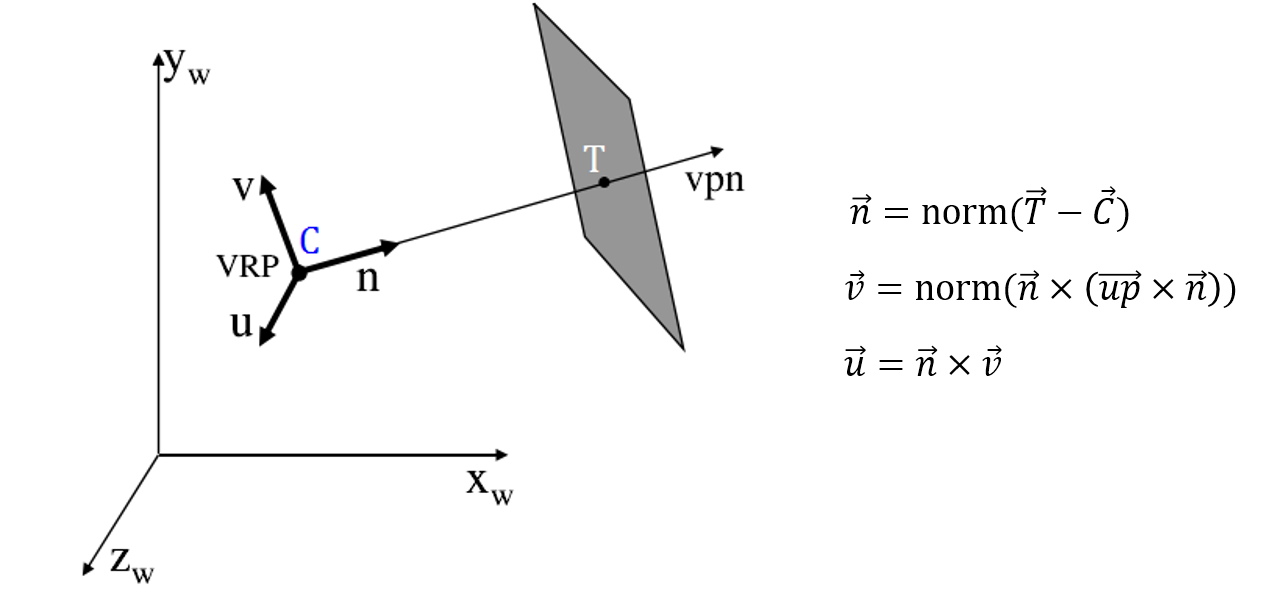
\includegraphics[width=\textwidth]{images/9Tgb3.png}
			\caption{uvn-система}
		\end{figure}
		}
	\end{frame}

	\begin{frame}{Преобразования наблюдения}

		\[
			M_{view} = M_{t} \times M_{uvn}
	 \]

	 \[
		 M_{view} = 
		 \begin{bmatrix}
			 1 & 0 & 0 & 0 \\
			 0 & 1 & 0 & 0 \\
			 0 & 0 & 1 & 0 \\
			 -p_x & -p_y & -p_z & 1 \\
		 \end{bmatrix}	
		 \begin{bmatrix}
			 u_x & u_y & u_z & 0 \\
			 v_x & v_y & v_z & 0 \\
			 n_x & n_y & n_z & 0 \\
			 0 & 0 & 0 & 1 \\
		 \end{bmatrix}	
		 =
	 \]

	 \[
		 =
		 \begin{bmatrix}
			 u_x & u_y & u_z & 0 \\
			 v_x & v_y & v_z & 0 \\
			 n_x & n_y & n_z & 0 \\
			 -p_x & -p_y & -p_z & 1 \\
		 \end{bmatrix}	
	 \]

		\note{

		\begin{figure} 
			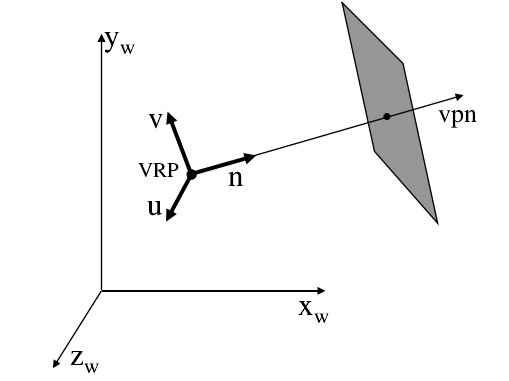
\includegraphics[width=0.65\textwidth]{images/ooEFp.png}
			\caption{uvn-система}
		\end{figure}


		}
	\end{frame}


	\section{Преобразование проецирования}

	\begin{frame}{Ортографическое проецирование}
		glm::ortho(float left, float right, float bottom, float top, float near, float far);
		
		Аргументы функции:
		\begin{itemize}
			\item 
			left, right расположены на оси x
			\item 
			bottom, top расположены на оси y
			\item 
			near, far расположены на оси z
		\end{itemize}

		Примечание.

		Параллельные линии остаются параллельными,
		\\ но при этом пропадает ощущение глубины, т.е. близко и далеко расположенные объекты относительно камеры имеют одинаковые размеры.
		\\ Все, что находится за пределами границы ортографической проекции, отсекается.


		\note{

		\begin{figure} 
			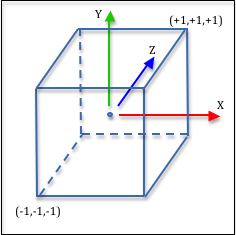
\includegraphics[width=0.5\textwidth]{images/clipping_volume.png}
			\caption{Граница ортографической проекции (куб)}
		\end{figure}

		}
	\end{frame}
	
	\begin{frame}{Ортографическое проецирование}
	
		Этапы преобразований
	\begin{enumerate}
		\item
		Центрирование границ ортографической проекции относительно начала системы координат в зависимости от заданных параметров.
		\item
		Масштабирование границ ортографической проекции так, чтобы получился куб с размерами сторон, равными 2.
		\item 
		Изменение направления оси z на противоположное, чтобы она соответствовала системе координат отсекающего пространства.
	\end{enumerate}



\end{frame}
	\begin{frame}{Ортографическое проецирование}
		
		1. Центрирование границ ортографической проекции относительно начала системы координат в зависимости от заданных параметров.

		\[
			c_x = \frac{left + right}{2}
		\]
		\[
			c_y = \frac{bottom + top}{2}
		\]
		\[
			c_z = - \frac{near + far}{2}
		\]

		\[
			M_t = 
			\begin{bmatrix}
				1 & 0 & 0 & 0 \\
				0 & 1 & 0 & 0 \\
				0 & 0 & 1 & 0 \\
				-c_x & -c_y & -c_z & 1 \\
			\end{bmatrix}	
		\]

		\note{
			Параметрическое уравнение прямой в пространстве
		\[
			\begin{cases}
				x = x_l + (x_r-x_l) t \\
				y = y_b + (y_t-y_b) t \\
				z = z_n + (z_f-z_n) t \\
			\end{cases}
		\]
		Параметрическое уравнение прямой в пространстве
		\[
			\begin{cases}
				x = (1 - t) x_l + x_r t \\
				y = (1 - t) y_b + y_t t \\
				z = (1 - t) z_n + z_f t \\
			\end{cases}
		\]


		% Параллельные линии модели остаются параллельным при отрисовке.

		% Два одинаковых объекта вне зависимости от расстояния от камеры одинаковы при отрисовке.

		% понятны значения параметров.
		
		% нужно отсечь все, что не лежит в области (-1,1)
		}
	\end{frame}

	\begin{frame}{Ортографическое проецирование}
		2. Масштабирование границ ортографической проекции так, чтобы получился куб с размерами сторон, равными 2.
		\[
			s_x = \frac{2}{right - left}
		\]
		\[
			s_y = \frac{2}{top - bottom}
		\]
		\[
			s_z =  \frac{2}{far - near}
		\]

		\[
			M_s = 
			\begin{bmatrix}
				s_x & 0 & 0 & 0 \\
				0 & s_y & 0 & 0 \\
				0 & 0 & s_z & 0 \\
				0 & 0 & 0 & 1 \\
			\end{bmatrix}	
		\]
		\note{
			Чтобы значения были в диапазоне от -1 до 1

		}
	\end{frame}	

	\begin{frame}{Ортографическое проецирование}
		3. Изменение направления оси z на противоположное, чтобы она соответствовала системе координат отсекающего пространства.
		\[
			M_{lh} = 
			\begin{bmatrix}
				1 & 0 & 0 & 0 \\
				0 & 1 & 0 & 0 \\
				0 & 0 & -1 & 0 \\
				0 & 0 & 0 & 1 \\
			\end{bmatrix}	
			\]
			\note{
				Левосторонняя система координат (left hand)
				
				inversion z-axis
		}	
			
	\end{frame}

	\begin{frame}{Ортографическое проецирование}
		\[
			M_t M_s M_{lh} =
		\]

		\[
			=
			\begin{bmatrix}
				\frac{2}{right - left} & 0 & 0 & 0 \\
				0 & \frac{2}{top - bottom} & 0 & 0 \\
				0 & 0 & -\frac{2}{far - near} & 0 \\
				-\frac{left + right}{right - left} & -\frac{bottom + top}{top - bottom} &  \frac{near + far}{far - near} & 1 \\
			\end{bmatrix}		
		\]
		\note{
			\[
				=
				\begin{bmatrix}
					1 & 0 & 0 & 0 \\
					0 & 1 & 0 & 0 \\
					0 & 0 & 1 & 0 \\
					-\frac{left + right}{2} & -\frac{bottom + top}{2} &  \frac{near + far}{2} & 1 \\
				\end{bmatrix}	
				\cdot
				\]
				\[
					\cdot
				\begin{bmatrix}
					\frac{2}{right - left} & 0 & 0 & 0 \\
					0 & \frac{2}{top - bottom} & 0 & 0 \\
					0 & 0 & \frac{2}{far - near} & 0 \\
					0 & 0 & 0 & 1 \\
				\end{bmatrix}	
				\begin{bmatrix}
					1 & 0 & 0 & 0 \\
					0 & 1 & 0 & 0 \\
					0 & 0 & -1 & 0 \\
					0 & 0 & 0 & 1 \\
				\end{bmatrix}	
				=
			\]
		}
	\end{frame}

	\begin{frame}{Перспективное проецирование}

		glm::perspective(float fovy, float aspect, float near, float far);
		
		glm::frustum(float left, float right, float bottom, float top, float near, float far);

		Примечание.

		Параллельные линии остаются параллельными,
		\\ но при этом пропадает ощущение глубины, т.е. близко и далеко расположенные объекты относительно камеры имеют одинаковые размеры.
		\\ Все что находится за пределами границы ортографической проекции отсекается.
		\note{
			\begin{figure} 
				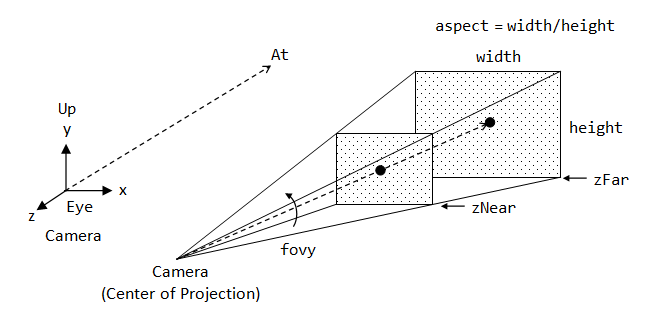
\includegraphics[width=\textwidth]{images/h15iq.png}
			\caption{Перспективная проекция}
		\end{figure}
		}
	\end{frame}

	\begin{frame}{Перспективное проецирование}{связь функций persective и frustum}

		
		glm::perspective(float fovy, float aspect, float near, float far);
		
		glm::frustum(float left, float right, float bottom, float top, float near, float far);
		
		Эти функции делают одно и тоже, но различаются аргументами.
		Переход от glm::frustum к glm::perspective имеет вид:

		Первый аргумент fovy  (field of view in y) обозначает «поле обзора по вертикали» (или угол обзора) и вычисляется как:
		\[
			fovy = 2 \cdot \arctan (top / near);
		\]
		Второй аргумент aspect (или aspectratio) обозначает «соотношение сторон» (отношение высоты к ширине, например, 16:9 или 4:3) и вычисляется как:
		\[
			aspect =  right / top
		\]
		
		\note{

			В дальнеем же будет применяться обратные преобразования, а именно:
			\[
			\text{top} = \text{near} \cdot \tan\left(\frac{\text{fovy}}{2}\right)
			\]

			\[
			\text{bottom} = -\text{top}
			\]

			\[
			\text{right} = \text{top} \cdot \text{aspect}
			\]

			\[
			\text{left} = -\text{right}
			\]

		}

	\end{frame}

	\begin{frame}{Перспективное проецирование}
		Этапы преобразований
		\begin{enumerate}
			\item Центрирование границ усеченной пирамиды относительно начала двумерной системы координат $XoY$.
			\item Масштабирование значения глубины $z$ в нормализованный диапазон $(-1, +1)$.
			\item Расчет перспективы.
			\item Масштабирование двумерных величин $(x', y')$ к квадратной области размером $[-1, 1]^2$
			% \item Измените направление оси $z$, чтобы соответствовать ориентации объема отсечения.
			\end{enumerate}

			\note{
				\begin{figure} 
					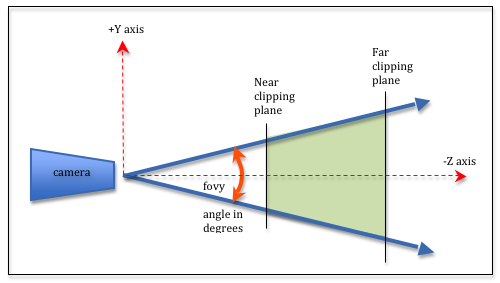
\includegraphics[width=0.9\textwidth]{images/side_view_frustum.png}
				\caption{Перспективная проекция}
			\end{figure}
			}

		\end{frame}

	\begin{frame}{Перспективное проецирование}
		1. Центрирование границ усеченной пирамиды относительно началы двумерной системы координат $XoY$.
		\[
			c_x = \frac{left + right}{2}
		\]
		\[
			c_y = \frac{bottom + top}{2}
		\]

		\[
			M_t = 
			\begin{bmatrix}
				1 & 0 & 0 & 0 \\
				0 & 1 & 0 & 0 \\
				0 & 0 & 1 & 0 \\
				-c_x & -c_y & 0 & 1 \\
			\end{bmatrix}	
		\]
	\end{frame}

	\begin{frame}{Перспективное проецирование}
		2. Масштабирование значения глубины $z$ в нормализованный диапазон $(-1, +1)$
		
В основе лежит нелинейное уравнение (модифицированное уравнение гиперболы) и имеет вид: 
\[
	z' = \frac{c_1}{-z} + c_2, 
\]
где $c_1$ и $c_2$ - это константы, которые вычисляются на основе диапазона $(-near, -far)$. 

Когда $z = -near$, уравнение должно давать $-1$. 
Когда $z = -far$, уравнение должно давать $+1$. 
Это дает нам два уравнения для решения $c_1$ и $c_2$.

\note{
	\begin{figure} 
		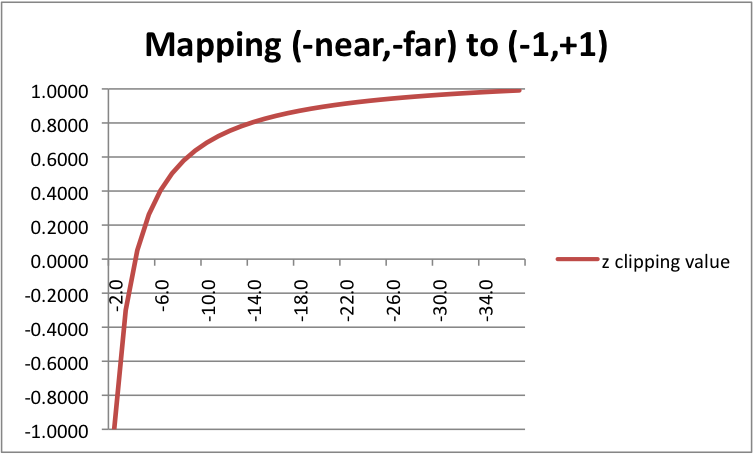
\includegraphics[width=0.75\textwidth]{images/non_linear_mapping.png}
	\caption{Кривая нелинейного уравнения}
\end{figure}


}
\end{frame}

\begin{frame}{Перспективное проецирование}

	В результате получаем следующую систему:

	\[
		\begin{cases}
			-1 = c_1/-(-near) + c_2 \\
			+1 = c_1/-(-far)  + c_2
		\end{cases}
	\]
	Т.е. получили СЛАУ, где $c_1$ и $c_2$ теперь неизвестные.
	\\
	Зная, чему равняются near и far в каждом частном случае, найдем константы $c_1$ и $c_2$.

	\[
		\begin{cases}
			c_1 = 2 far \cdot near / (near - far) \\
			c_2 = (far + near) / (far - near)
		\end{cases}
	\]

	Но куда же их подставлять в нашу матрицу?


		\note{
		%Мы уже вычислили правильное положение вершины на 2D окне просмотра, но мы еще не изменили компоненту z. 
		Нельзя просто отбросить значение z, так как оно указывает на расстояние между вершиной и камерой, что позволяет нам определить, какие объекты находятся перед другими. 
		Мы могли бы сделать линейное отображение между диапазоном (-near, -far) и (-1, +1). Однако числа с плавающей запятой подвержены погрешностям округления при выполнении математических операций. В графических приложениях иногда разница между 0.1234568 и 0.1234567 может оказать визуальное воздействие на рендеринг. Мы хотели бы использовать большую точность для значений, близких к камере, и меньшую точность для вершин, находящихся дальше от камеры. Это означает, что нам нужно нелинейное отображение между (-near, -far) и (-1, +1).
		}
	\end{frame}

	\begin{frame}{Перспективное проецирование}
	Рассмотрим правую часть нелинейного уравнения и вынесем знаменатель $-z$ за скобки:
		\[
		z' =  \frac{1}{-z} (-c2 \cdot z + c1)
	\]

	Используем матричные преобразования, чтобы перейти от конкретного значения $z$ к модифицированному значению $z'$:\\ 
	перемещение, т.е. прибавление $c1$, \\
	масштабирование, т.е. умножение на $-c2$, \\
	проецирование, т.е. деление $-z$.

	Тогда получим следующую матрицу.


	\[
		M_{sz} = 
	\begin{bmatrix}
		1 & 0 & 0 & 0 \\
		0 & 1 & 0 & 0 \\
		0 & 0 & -c_2 & -1 \\
		0 & 0 & c_1 & 0 \\
	\end{bmatrix}	
	\]

	\note{

	\[
		\begin{bmatrix}
			p_x \\
			p_y \\
			p_z \\
			1		\\
		\end{bmatrix}^T
		\begin{bmatrix}
			1 & 0 & 0 & 0 \\
			0 & 1 & 0 & 0 \\
			0 & 0 & -c_2 & -1 \\
			0 & 0 & c_1 & 0 \\
		\end{bmatrix}
		=
		\begin{bmatrix}
			p_x \\
			p_y \\
			-c_2 p_z + c_1 \\
			-z	\\
		\end{bmatrix}^T
		\]
		\[
			\begin{bmatrix}
				p_x^{*} \\
				p_y^{*} \\
				p_z^{*} \\
				1		\\
			\end{bmatrix}^T
			=
			\begin{bmatrix}
			 p_x / (-z) \\
				p_y / (-z) \\
				(-c_2 p_z + c_1) / (-z) \\
				1	\\
			\end{bmatrix}^T
		\]
	}

\end{frame}

	\begin{frame}{Перспективное проецирование}
		3. Расчет перспективы

		Пусть $(x, y, z)$ --- координаты вершины. \\ 
		Задача: отобразить на 2D окне просмотра.

    Спроецируем вершину на ближнюю плоскость окна просмотра, т.е. нужно перейти от $(x,y,z)$ к $(x',y',near)$. \\
		Интерпретация. \\
    Здесь $\text{near}$ - это значение, представляющее ближнюю плоскость отсечения. Значения $y$ и $z$ различаются для каждой вершины в сцене и представляют ее трехмерные координаты. Результатом этих вычислений будут координаты $(x', y', \text{near})$, которые представляют положение вершины на ближней плоскости окна просмотра.


		\note{
			\begin{figure} 
				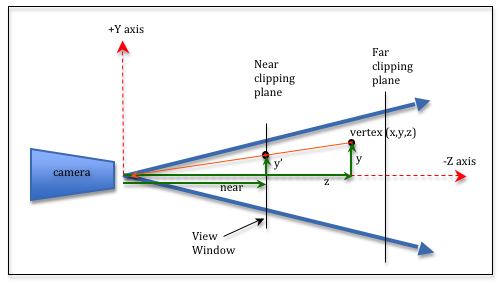
\includegraphics[width=0.9\textwidth]{images/perspective_divide.png}
			\caption{Схема смещения значений}
		\end{figure}
		}

	\end{frame}

	\begin{frame}{Перспективное проецирование}
		Тогда матрица будет иметь вид:
 \[
	M_p = 
	 \begin{bmatrix}
		near & 0 & 0 & 0 \\
		0 & near & 0 & 0 \\
		0 & 0 & 1 & 0 \\
		0 & 0 & 0 & 1 \\
	\end{bmatrix}	
	\]

	\note{
		Тогда можно составить следующие пропорции:
		\[
			\frac{x'}{x}  = \frac{-near}{z}
			\qquad
			\frac{y'}{y} = \frac{-near}{z}
		\]

		В результате получаем следующие формулы:
		\[
			x' = \frac {near}{-z} x
			\qquad
			y' = \frac{near}{-z} y
		\]

		Учитывая предыдущий шаг, получается, что не хватает лишь множителя $near$.
	}
	\end{frame}

	\begin{frame}{Перспективное проецирование}

		4. Масштабирование двумерных величин $(x', y')$ к квадратной области размером $[-1, 1]^2$

		\[
			s_x = \frac{2}{right - left}
		\]
		\[
			s_y = \frac{2}{top - bottom}
		\]

		\[
			M_{s2d} = 
			\begin{bmatrix}
				s_x & 0 & 0 & 0 \\
				0 & s_y & 0 & 0 \\
				0 & 0 & 1 & 0 \\
				0 & 0 & 0 & 1 \\
			\end{bmatrix}	
		\]
	\end{frame}

	\begin{frame}{Перспективное проектирование}
		\[
			M_t M_{sz} M_p M_{s2d} =
		\]

		\[
			=
			\begin{bmatrix}
				\frac{2 near}{right - left} & 0 & 0 & 0 \\
				0 & \frac{2 near}{top - bottom} & 0 & 0 \\
				0 & 0 & -\frac{far + near}{far - near} & -1 \\
				-near \frac{right + left}{right - left} & -near \frac{top+ bottom}{top - bottom} & \frac{2 near \cdot far}{near - far} & 0 \\
			\end{bmatrix}		
		\]
		\note{
			Промежуточные расчеты

			\[
				=
				\begin{bmatrix}
					1 & 0 & 0 & 0 \\
					0 & 1 & 0 & 0 \\
					0 & 0 & 1 & 0 \\
					-\frac{left + right}{2} & -\frac{bottom + top}{2} & 0 & 1 \\
				\end{bmatrix}	
				\begin{bmatrix}
					1 & 0 & 0 & 0 \\
					0 & 1 & 0 & 0 \\
					0 & 0 & - \frac{far + near}{far - near} & -1 \\
					0 & 0 & \frac{2 far \cdot near} {near - far} & 0 \\
				\end{bmatrix}	
				\cdot
				\]
				\[
					\cdot
				\begin{bmatrix}
					near & 0 & 0 & 0 \\
					0 & near & 0 & 0 \\
					0 & 0 & 1 & 0 \\
					0 & 0 & 0 & 1 \\
				\end{bmatrix}	
				\begin{bmatrix}
					\frac{2}{right - left} & 0 & 0 & 0 \\
					0 & \frac{2}{top - bottom} & 0 & 0 \\
					0 & 0 & 1 & 0 \\
					0 & 0 & 0 & 1 \\
				\end{bmatrix}	
				=
			\]
		}
	\end{frame}

	

	\end{document}
	
	% https://learnwebgl.brown37.net/08_projections/projections_ortho.html
	% https://www.songho.ca/opengl/gl_projectionmatrix.html
	% https://www.scratchapixel.com/lessons/3d-basic-rendering/perspective-and-orthographic-projection-matrix/opengl-perspective-projection-matrix.html
	% https://en.wikipedia.org/wiki/Viewing_frustum
	% https://www.reddit.com/r/opengl/comments/2hs6cf/questionglmfrustum_or_glmperspective/
	% https://startandroid.ru/ru/uroki/vse-uroki-spiskom/401-urok-172-perspective-frustum-ortho.html
	% http://doc.51windows.net/Directx9_SDK/graphics/programmingguide/fixedfunction/viewportsclipping/viewingfrustum.htm
	% https://www.google.com/search?q=camera+transformation+FOV&tbm=isch&ved=2ahUKEwjh6-yX7_CBAxXwBxAIHS7gDtwQ2-cCegQIABAA&oq=camera+transformation+FOV&gs_lcp=CgNpbWcQAzoHCAAQigUQQzoFCAAQgAQ6BggAEAgQHjoHCAAQGBCABDoECAAQHlDSAlizDWDWDmgBcAB4AIABUYgBwwKSAQE2mAEAoAEBqgELZ3dzLXdpei1pbWfAAQE&sclient=img&ei=mxYoZaGyMvCPwPAPrsC74A0&bih=921&biw=1920#imgrc=1JjqcwhhFgAhiM



	\begin{figure} 
		\href{https://www.researchgate.net/figure/Outline-of-the-graphics-pipeline_fig1_281810652}{
			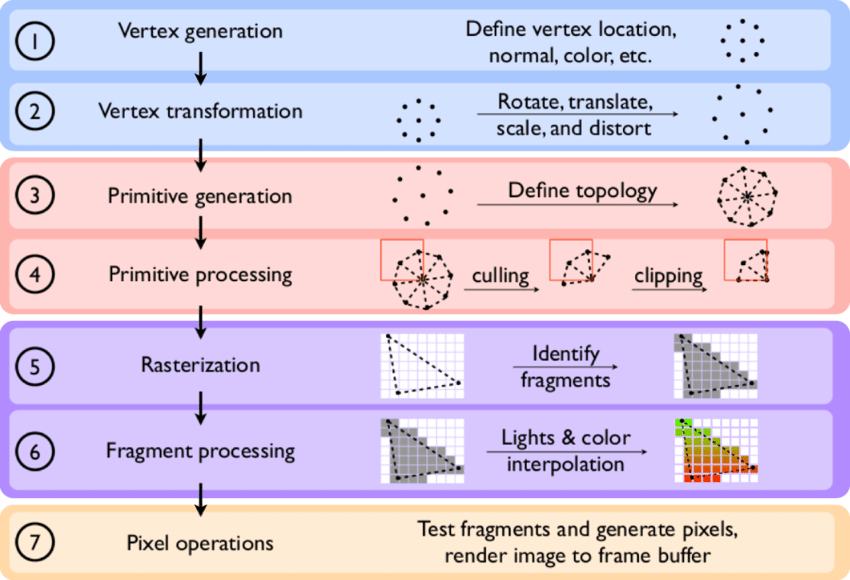
\includegraphics[width=0.75\textwidth]{images/Outline-of-the-graphics-pipeline.png}}
		\caption{Схема графического конвейера}
	\end{figure}

	\begin{figure} 
			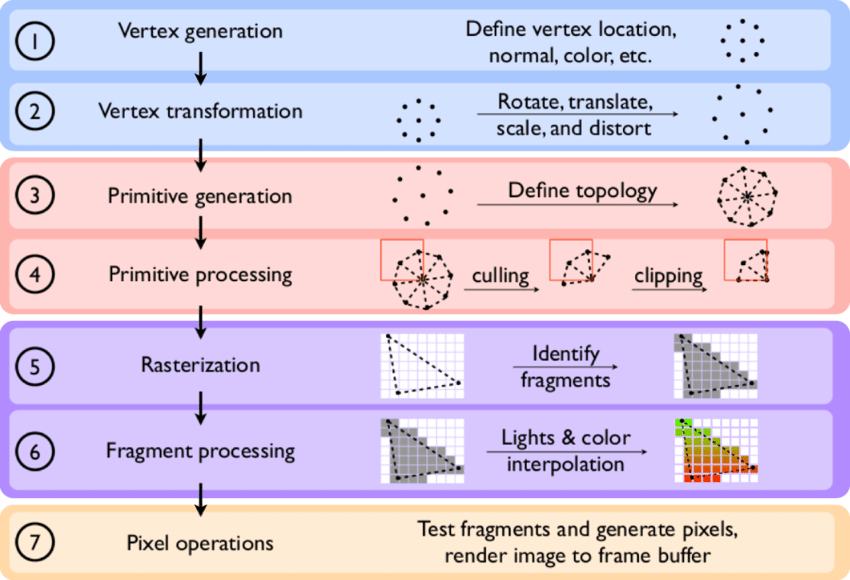
\includegraphics[width=0.75\textwidth]{images/Outline-of-the-graphics-pipeline.png}
		\caption{Схема графического конвейера}
	\end{figure}

	\begin{columns}
		\begin{column}{0.5\textwidth}
			\begin{figure} 
				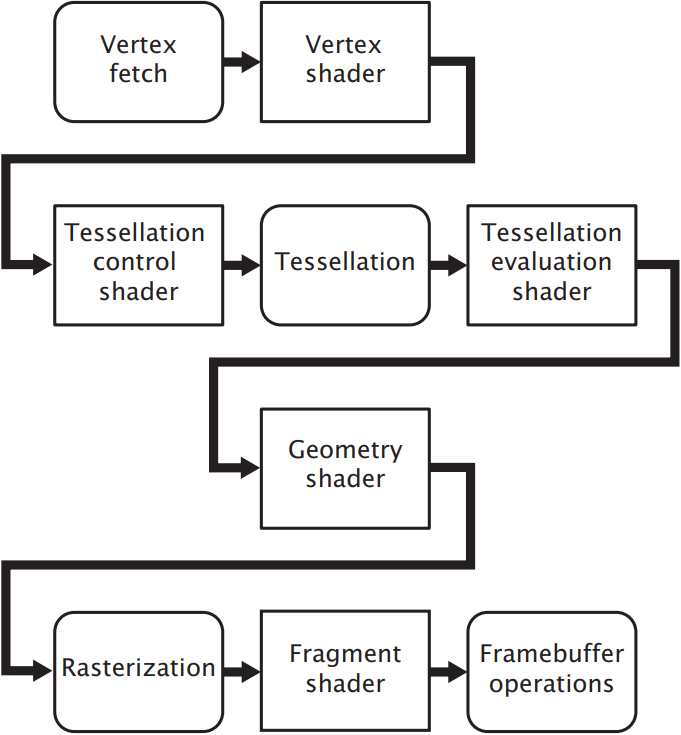
\includegraphics[width=0.9\textwidth]{images/Simplified_model_of_the_graphics_pipeline.png}
				\caption {Порядок вычисления шейдеров}
			\end{figure}
		\end{column}
		\begin{column}{0.5\textwidth}
		\end{column}
	\end{columns}
			

			\footnotesize

			\begin{table}
				% \caption{\label{tab:fractal} Название}
				\begin{center}
					\begin{tabular}{|c|c|c|}
						\hline
						$k$ & $l$ & $N(l)$ \\
						\hline
						0 & $1$ & $1$ \\
						\hline
						1 & $1/2$ & $3$ \\
						\hline
						2 & $1/4$ & $9$ \\
						\hline
						\multicolumn{3}{|c|} {\dots} \\
						\hline
						n & $2^{-n}$ & $3^{n}$ \\
						\hline
					\end{tabular}
				\end{center}
			\end{table}